\documentclass[11pt,fleqn,dvipsnames,usenames]{article}

% to keep this file less overwhelming

\usepackage[version=4]{mhchem}

% Where to look for pngs and jpegs
\graphicspath{{Images//}}

\usepackage[includehead, includefoot, left= 2cm, top =1.5cm, bottom = 1.5cm, textwidth=17.5cm]{geometry}

\usepackage{pifont, amsmath}

% packages to include

\usepackage[dvipsnames, table]{xcolor}

\usepackage{
  amsmath,
  amssymb, 
  arydshln, % for hyphenated lines in block matrices
  fancyhdr, % needed for header at top of each page
  graphicx, % to include pictures
  hyperref, % for hyper links
  mathtools, % for a longer arrow
  multicol, % displaying enumerates and itemizes into multiple columns
  multirow, % for tables
  multido, % for TOC
  pgfplots, % for axis environment within tikz pictures
  systeme,
  tikz,
}

\usepackage[inline, shortlabels]{enumitem}


% global constants
\newcommand{\term}{Fall 2024}
\newcommand{\course}{Math 2210}

% mathbb aliases
\newcommand{\COMPLEX}{\mathbb{C}}
\newcommand{\C}{\COMPLEX}
\newcommand{\REAL}{\mathbb{R}}
\newcommand{\R}{\REAL}
\newcommand{\RATIONAL}{\mathbb{Q}}
\newcommand{\Q}{\RATIONAL}
\newcommand{\INTEGER}{\mathbb{Z}}
\newcommand{\Z}{\INTEGER}
\newcommand{\ZN}{\INTEGER_{n}}
\newcommand{\NATURAL}{\mathbb{N}}
\newcommand{\N}{\NATURAL}

\newcommand{\ZX}{\Z[x]}
\newcommand{\ZNX}{\ZN[x]}
\newcommand{\QX}{\Q[x]}
\newcommand{\RX}{\R[x]}
\newcommand{\CX}{\C[x]}
\newcommand{\CZ}{\C[z]}

% complex number aliases
\newcommand{\RE}[1]{\text{Re}\left(#1\right)}
\newcommand{\IM}[1]{\text{Im}\left(#1\right)}
\newcommand{\CC}[1]{\overline{#1}}
\newcommand{\ARG}[1]{\text{arg}\left(#1\right)}
\newcommand{\PARG}[1]{\text{Arg}\left(#1\right)}

% for financial stuff
\newcommand{\dollar}{\mathrm{\$}}

% nicer looking trig functions
\newcommand{\SIN}[1]{\sin\left(#1\right)}
\newcommand{\COS}[1]{\cos\left(#1\right)}
\newcommand{\TAN}[1]{\tan\left(#1\right)}
\newcommand{\CSC}[1]{\csc\left(#1\right)}
\newcommand{\SEC}[1]{\sec\left(#1\right)}
\newcommand{\COT}[1]{\cot\left(#1\right)}

% number theory
\newcommand{\ndiv}{|\kern-0.9ex{/}}

% automatically resize set brackets
\newcommand{\SET}[1]{\left\{#1\right\}}

% sums and products
\newcommand{\SUM}{\displaystyle\sum\limits}
\newcommand{\PROD}{\displaystyle\prod\limits}
\newcommand{\LIMIT}{\displaystyle\lim\limits}
\newcommand{\of}{\circ}
\newcommand{\restrict}[1]{\raisebox{-.5ex}{$|$}_{#1}}

% set intersection and union
\newcommand{\CAP}{\displaystyle\bigcap\limits}
\newcommand{\CUP}{\displaystyle\bigcup\limits}

% polynomials
\newcommand{\DEG}[1]{\ensuremath{\text{deg}\left(#1\right)}}

% max and min
\newcommand{\MAX}[1]{\ensuremath{\max\left\{#1\right\}}}
\newcommand{\MIN}[1]{\ensuremath{\min\left\{#1\right\}}}

% gcd and lcm
\newcommand{\GCD}[1]{\ensuremath{\text{gcd}\left(#1\right)}}
\newcommand{\LCM}[1]{\ensuremath{\text{lcm}\left(#1\right)}}

% for writing logic within mathematics environment
\newcommand{\FORALL}{\ensuremath{\text{ for all }}}
\newcommand{\FORSOME}{\ensuremath{\text{ for some }}}

% matrix notation
\newcommand{\MATRIX}[2]{\ensuremath{\left[\begin{array}{#1}#2\end{array}\right]}}
\newcommand{\COLUMN}[1]{\ensuremath{\left[\begin{array}{r}#1\end{array}\right]}}
\newcommand{\BY}{\times}

% vector notation
%\newcommand{\vv}{\overset{\rightharpoonup}}
\newcommand{\vv}[1]{{\bf #1}}
\newcommand{\arr}{\overrightarrow}

% dot product
\newcommand{\dotp}{{\scriptstyle\bullet}}

% Text macros
\newcommand{\KER}[1]{\ensuremath{\text{ker}\left(#1\right)}}
\newcommand{\IMG}[1]{\ensuremath{\text{im}\left(#1\right)}}
\newcommand{\CHAR}[1]{\ensuremath{\text{char}\left(#1\right)}}
\newcommand{\BIGO}[1]{\ensuremath{\mathcal{O}\left(#1\right)}}
\newcommand{\TR}[1]{\ensuremath{\text{tr}\left(#1\right)}}

% abbreviations
\newcommand{\ds}{\displaystyle}
\newcommand{\md}{\mdseries}

% abbreviations for vertical/horizontal spaces
\newcommand{\vsp}{\vspace{0.5cm}}
\newcommand{\smsp}{\vspace{0.25cm}} % small space
\newcommand{\vsmsp}{\vspace{0.1cm}} % very small space
\newcommand{\hsp}{\hspace{0.25cm}}

% new operators
\DeclareMathOperator\SPAN{Span}
\newcommand{\SPANOF}[1]{\ensuremath{\SPAN\left\{#1\right\}}}
\DeclareMathOperator\PROJ{proj}
\DeclareMathOperator\PERP{perp}

% underlining definitions
\newcommand{\DEF}[1]{\textbf{\ul{#1}}}

% environments
\newtheorem{theorem}{Theorem}[subsection]
\newtheorem*{theorem*}{Theorem}
\newtheorem{corollary}[theorem]{Corollary}
\newtheorem*{corollary*}{Corollary}
\newtheorem{lemma}[theorem]{Lemma}

\theoremstyle{definition}
\newtheorem{definition}[theorem]{Definition}
\newtheorem*{definition*}{Definition}
\newtheorem{example}[theorem]{Example}
\newtheorem*{example*}{Example}
\newtheorem{examples}[theorem]{Examples}
\newtheorem*{examples*}{Examples}
\newtheorem{exercise}[theorem]{Exercise}
\newtheorem*{exercise*}{Exercise}
\newtheorem{exercises}[theorem]{Exercises}
\newtheorem{remark}[theorem]{Remark}
\newtheorem{remarks}[theorem]{Remarks}

% make proof boxes solid
\renewcommand{\qedsymbol}{$\blacksquare$}

% quick abbreviations to avoid using latex environments (gradually phasing these out)
\newcommand{\analogy}{\noindent \textbf{Analogy:} }
\newcommand{\answer}{\noindent \textbf{Answer:} }
\newcommand{\answers}{\noindent \textbf{Answers:} }
\newcommand{\application}{\noindent \textbf{Application:} }
\newcommand{\background}{\noindent \textbf{Background:} }
\newcommand{\caution}{\noindent \textbf{Caution:} }
\newcommand{\conclusion}{\noindent \textbf{Conclusion:} }
\newcommand{\consequence}{\noindent \textbf{Consequence:} }
\newcommand{\convention}{\noindent \textbf{Convention:} }
\newcommand{\conventions}{\noindent \textbf{Conventions:} }
\newcommand{\crlry}{\noindent \textbf{Corollary:} }
\newcommand{\defn}{\noindent \textbf{Definition:} }
\newcommand{\details}{\noindent \textbf{Details:} }
\newcommand{\nexamples}[1]{\noindent \textbf{Examples (#1):}} 
\newcommand{\exception}{\noindent \textbf{Exception:} }
\newcommand{\nexercise}[1]{\noindent \textbf{Exercise (#1):}} 
\newcommand{\nexercises}[1]{\noindent \textbf{Exercises (#1):}} 
\newcommand{\fact}{\noindent \textbf{Fact:} }
\newcommand{\facts}{\noindent \textbf{Facts:} }
\newcommand{\fix}{\noindent \textbf{Fix:} }
\newcommand{\formula}{\noindent \textbf{Formula:} }
\newcommand{\goal}{\noindent \textbf{Goal:} }
\newcommand{\goals}{\noindent \textbf{Goals:} }
\newcommand{\hint}{\noindent \textbf{Hint:} }
\newcommand{\idea}{\noindent \textbf{Idea:} }
\newcommand{\illustration}{\noindent \textbf{Illustration:} }
\newcommand{\important}{\noindent \textbf{Important:} }
\newcommand{\lema}{\noindent \textbf{Lemma:} }
\newcommand{\midea}{\noindent \textbf{Main Idea:} }
\newcommand{\motivation}{\noindent \textbf{Motivation:} }
\newcommand{\nthm}[1]{\noindent \textbf{Theorem} (\textit{#1}):}
\newcommand{\notation}{\noindent \textbf{Notation:} }
\newcommand{\note}{\noindent \textbf{Note:} }
\newcommand{\notes}{\noindent \textbf{Notes:} }
\newcommand{\observation}{\noindent \textbf{Observation:} }
\newcommand{\observations}{\noindent \textbf{Observations:} }
\newcommand{\pict}{\noindent \textbf{Picture:} }
\newcommand{\plan}{\noindent \textbf{Plan:} }
\newcommand{\prf}{\noindent \textbf{Proof:} }
\newcommand{\problem}{\noindent \textbf{Problem:} }
\newcommand{\properties}{\noindent \textbf{Properties:} }
\newcommand{\question}{\noindent \textbf{Question:} }
\newcommand{\questions}{\noindent \textbf{Questions:} }
\newcommand{\recall}{\noindent \textbf{Recall:} }
\newcommand{\reason}{\noindent \textbf{Reason:} }
\newcommand{\reminder}{\noindent \textbf{Reminder:} }
\newcommand{\solution}{\noindent \textbf{Solution:} }
\newcommand{\nsolution}[1]{\noindent \textbf{Solution #1:} }
\newcommand{\setting}{\noindent \textbf{Setting:} }
\newcommand{\strategy}{\noindent \textbf{Strategy:} }
\newcommand{\summary}{\noindent \textbf{Summary:} }
\newcommand{\terminology}{\noindent \textbf{Terminology:} }
\newcommand{\thm}{\noindent \textbf{Theorem:} }
\newcommand{\work}{\noindent \textbf{Work:} }

% gray line across pagewidth
\newcommand{\GRAYLINE}{
  {\color{gray}\leaders\vrule width \textwidth\vskip0.4pt} % or other desired thickness
  \vskip\medskipamount % ditto
  \nointerlineskip
  \smsp
}

% used when adding fill-in-the-blanks for students
\newcommand{\blank}[1]{\underline{\hspace{#1}}}

% indents annoy me, and so does repeatedly typing \noindent
\newcommand{\p}{\noindent}

\begin{document}

\begin{enumerate}

\item[1.] For Adrienne not to know the birthday immediately, the number could not be any of $3, 20$ or $26$.  Since Nicole knew this, she must have been told that the month was either May or September.  Adrienne also arrives at this conclusion, and somehow determines the month.  This tells Nicole that the birthday must be September 1st, September 16th, or March 28th.  Since she still does not know the birthday, it must September 1st or 16th and the correct answer is (D).

\item[3.] The prime factorization of $3^{14} + 3^{13} - 12$ may be computed as
\begin{align*}
3^{14} + 3^{13} - 12 &= 3(3^{13} + 3^{12} - 4)\\
&=  3(3^{12}\cdot 4 - 4)\\
&=  3\cdot 4\cdot (3^{12}-1)\\
&=  2^2\cdot 3\cdot(3^{6} -1)(3^{6} + 1)\\
&=  2^2\cdot 3\cdot(3^3 - 1)(3^3 + 1)(3^{6} + 1)\\
&=  2^2\cdot 3\cdot 26\cdot 28\cdot (3^{6} + 1)\\
&=  2^5\cdot 3\cdot 7\cdot 13\cdot (3^{6} + 1)\\
&=  2^5\cdot 3\cdot 7\cdot 13\cdot 730\\
&=  2^6\cdot 3\cdot 5\cdot 7\cdot 13\cdot 73\\
\end{align*}

Hence $73$ is the largest prime divisor and the correct answer is (E).

\item[5.] Since $x + y + z = 1$, we must have also have $(x + y + z)^2 = 1$.  So
\begin{align*}
1 &= (x + y + z)^2\\
&= x^2 + xy + xz + yx + y^2 + yz + zx + zy + z^2\\
&= x^2 + y^2 + z^2 + 2(xy + zy + yz)\\
&= 3 + 2(xy + zy + yz).
\end{align*}
Therefore $xy + zy + yz = \frac{1-3}{2} = -1$ and the correct answer is (B).

\item[6.] \p \bf Suggestion: \md The first time I solved this problem, I got $r$ and $t$ reversed because I misinterpreted the problem.  This was my own fault, but the chances of this happening might be reduced if we replace `in opposite directions' with `towards eachother'.

Let $s_{1}$ and $s_{2}$ be the speeds of the faster and slower cyclist, respectively.  It is given that
\begin{center}
$s_{1} + s_{2} = k/t$ and $s_{1} - s_{2} = r/t$.
\end{center}
Adding and subtracting these equations yields
\begin{center}
$2s_{1} = \dfrac{k}{t} + \dfrac{r}{t}$ and $2s_{2} = \dfrac{k}{t} - \dfrac{r}{t}$.
\end{center}
Hence
\begin{center}
$\dfrac{s_{1}}{s_{2}} = \dfrac{2s_{1}}{2s_{2}} = \dfrac{\frac{k}{t} + \frac{r}{t}}{\frac{k}{t} - \frac{r}{t}} = \dfrac{r+t}{r-t}$,
\end{center}
making (A) the correct answer.

\item[7.] There are two distinct \emph{paths} from A to B (shown below in red), each of which may be extended with two optional loops (shown below in blue).
\begin{center}
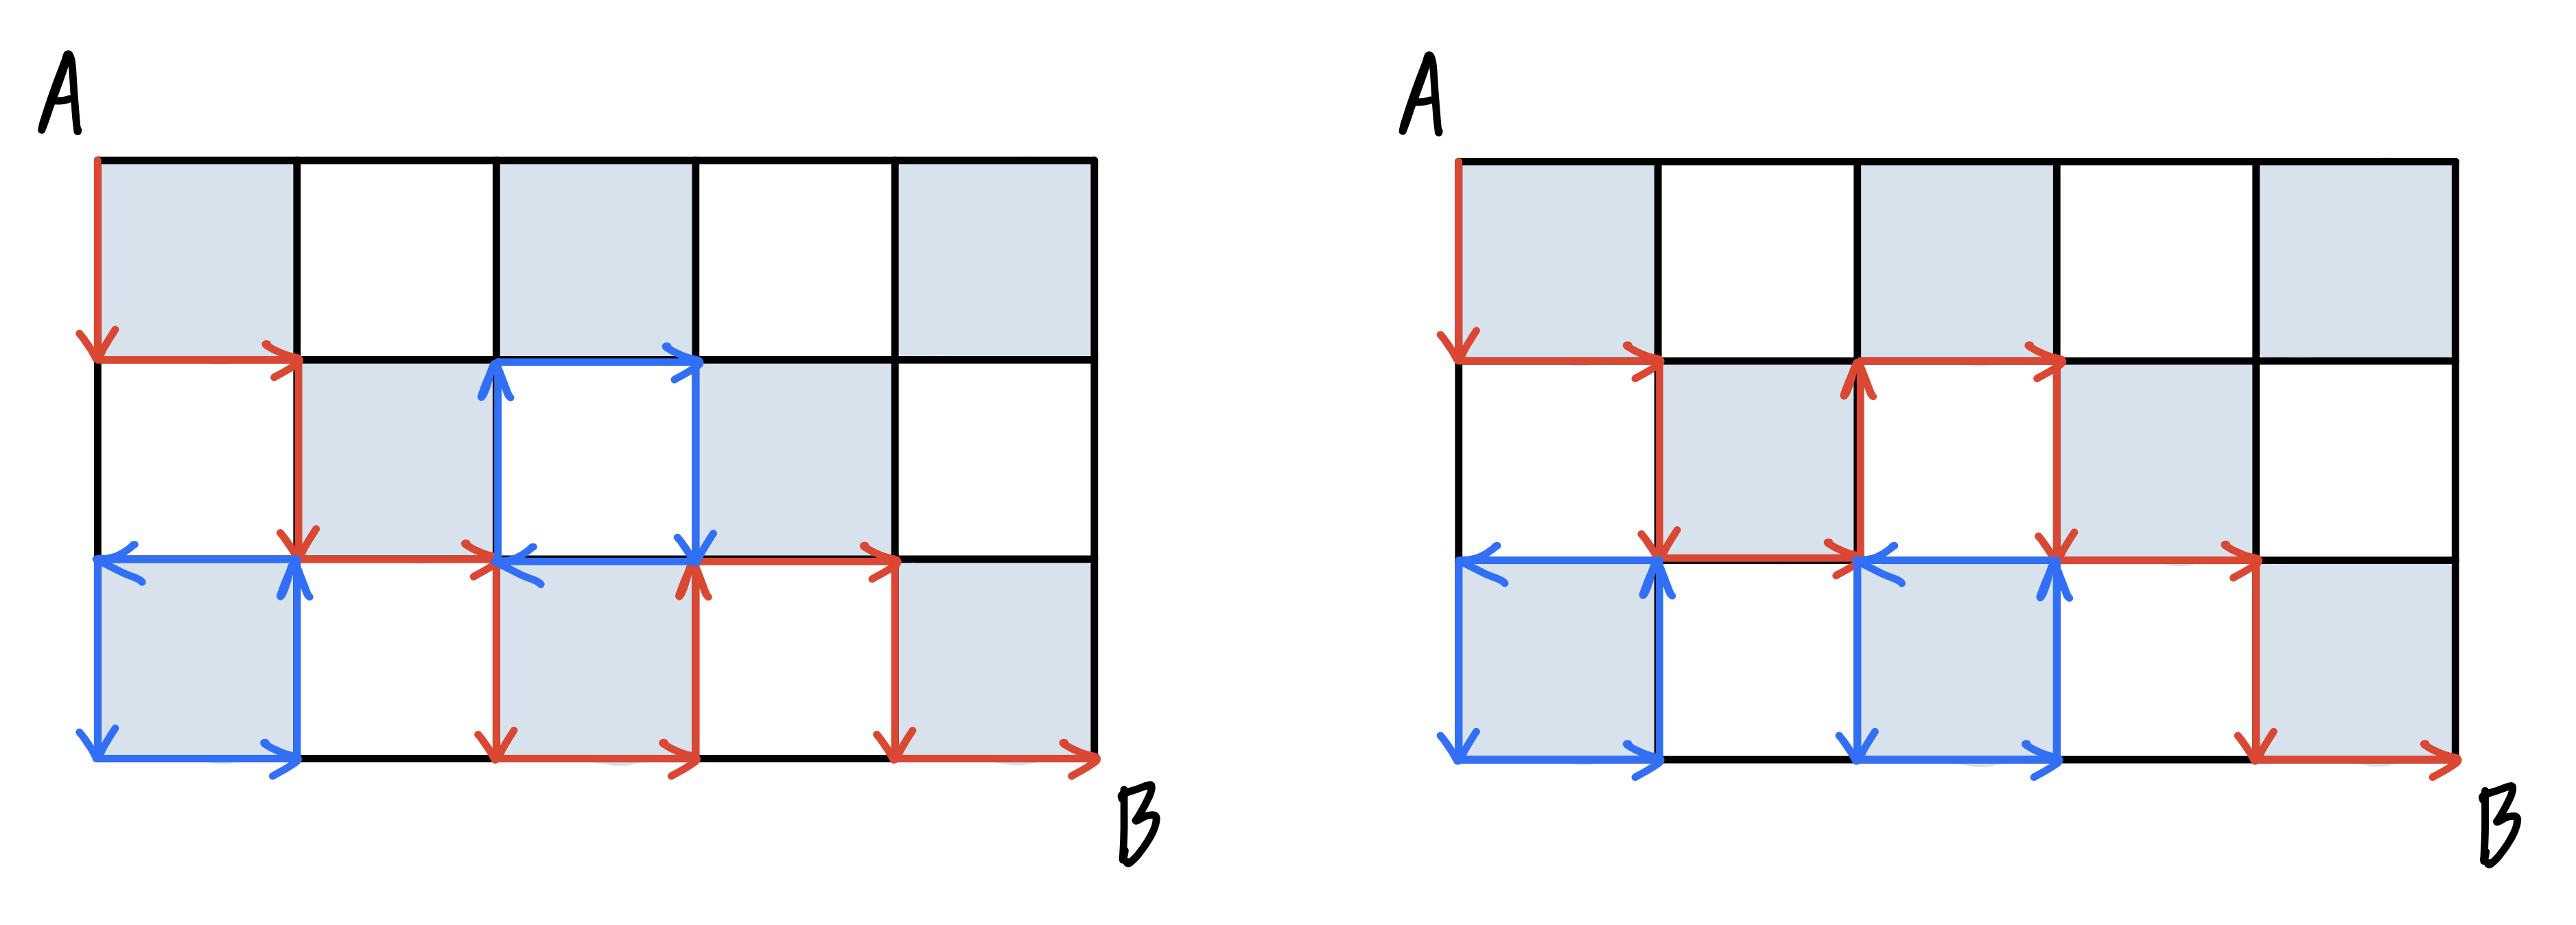
\includegraphics[width=0.8\linewidth]{routes}
\end{center}
To avoid double-counting, insist that blue edges are traversed with priority.  Considering each blue loop as optional, there are four possible variations of each path, and hence 8 possibilities in total.

\item[9.] \note It seems that the requirement is satisfied if $k=0$, which may have been unintentional.  If a unique answer is desired, it should be explicitly required that $k>0$.

For $j=1,2$, let each of $R_{j}, G_{j}$ and $B_{j}$ respectively denote the events that a red, green, or ball is chosen for the first and second drawn card.  The probability that both cards are the same colour is given by
\begin{center}
$\dfrac{3}{9+k}\cdot\dfrac{2}{8 + k} + \dfrac{6}{9+k}\cdot\dfrac{5}{9+k} + \dfrac{k}{9+k}\cdot\dfrac{k-1}{8+k} = \dfrac{36 - k + k^2}{(9+k)(8+k)}$.
\end{center}
%
The probability that each card is a different colour is given by
\begin{center}
$\dfrac{3}{9+k}\cdot \dfrac{6+k}{8+k} + \dfrac{6}{9+k}\cdot \dfrac{3+k}{8+k} + \dfrac{k}{9+k}\cdot \dfrac{9}{8+k} = \dfrac{36 + 18k}{(9+k)(8+k)}$.
\end{center}
By assumption, these probabilities are equal, which means that $36 + 18k = 36 - k + k^2$, which is true when $k = 0$ or $k=19$.

\item[10.] \note I could not reproduce any of the answers listed, and if there is an error in my logic below, I can't find it.  Let me know what you think!

Let $A_{1}$ and $A_{2}$ be the event that each of the first and second cards drawn are aces, respectively.

First note that
\begin{itemize}
\item $P(A_{1}) = \dfrac{4}{16} = \dfrac{1}{4}$,
\item $P(A_{2}) = P(A_{2}|A_{1}) + P(A_{2}|A_{1}^{c}) = \dfrac{3}{15} + \dfrac{4}{15} = \dfrac{7}{15}$, and
\item $P(A_{1}\cap A_{2}) = P(A_{1})P(A_{2}|A_{1}) = \dfrac{1}{4}\cdot \dfrac{3}{15} = \dfrac{1}{20}$.
\end{itemize}
So the desired probability is
\begin{align*}
P(A_{1}\cap A_{2}|A_{1}\cup A_{2}) &= \dfrac{P\big((A_{1}\cap A_{2})\cap (A_{1}\cup A_{2})\big)}{P(A_{1}\cup A_{2})}\\
&= \dfrac{P(A_{1}\cap A_{2})}{P(A_{1}) + P(A_{2}) - P(A_{1}\cap A_{2})}\\
&= \dfrac{1/20}{1/4 + 7/15 - 1/20}\\
&= \dfrac{3}{15 + 28 - 3}\\
&= \dfrac{3}{40}
\end{align*}
\end{enumerate}
\end{document}





